\label{sec:noisy_adders}
In this section, we are describing a noise model based on the assumption that the input voltage to the actual circuit implementing the logic NAND, NOR or NOT gates are no longer kept constant resulting in variation of the {\em actual value} of the input to the NAND, NOR or NOT unit (see \cite{LiMunPat2006l} for related work on the NOT-gate). Looking at the electrical circuit diagram of a CMOS NOT-, NAND- or NOR-gate in Figure \ref{fig:not-nand-nor-CMOS}, we see that such a variation would alter the input voltage $V_i$ thereby leading to switching behavior of the corresponding MOSFET transistors.

We assume that the random variation is fully described through two parameters $\alpha \in \left[0,\frac{1}{2}\right]$ and $\beta \in \left[0,\frac{1}{2}\right]$ which denote the probability that a low-voltage input (i.e., bit state of $0$) switches the n-type MOSFET on (i.e., bit state of $1$) and vice versa for the p-type MOSFET\footnote{Note that a flip probability of more than 50\% means that the inverted gate would make less mistakes.}. More formally, we assume that
\begin{align}
    P(a_\text{obs} = 1 | a = 0) & = \alpha\,, \label{eq:bit_flip_to_1} \\
    P(a_\text{obs} = 0 | a = 1) & = \beta\,. \label{eq:bit_flip_to_0}
\end{align}
With this noise model, it is possible that an NAND, NOR or NOT gate make mistakes in their computation. In the following table, we have listed the respective probability of each outcome $0$ and $1$ for the full list of bit-wise inputs $a$ and $b$.

\begin{center}
    \begin{tabular}{c|c||c|c||c|c||c|c}
        \multicolumn{2}{c||}{}         &
        $P\left(a \land b = 1\right)$  & $P\left(a \land b = 0\right)$  &
        $P\left(a \lor b = 1\right)$   & $P\left(a \lor b = 0\right)$   &
        $P\left(\neg a = 0\right)$     & $P\left(\neg a = 1\right)$       \\
        \hline
        $a$                            & $b$                            &
        $q_\NAND(a,b,0)$               & $q_\NAND(a,b,1)$               &
        $q_\NOR(a,b,0) $               & $q_\NOR(a,b,1)$                &
        $q_\NOT(a,0)$                  & $q_\NOT(a,1)$                    \\
        \hline
        $0$                            & $0$                            &
        $\alpha^2$                     & $1-\alpha^2$                   &
        $1-\left(1-\alpha\right)^2$    & $\left(1-\alpha\right)^2$      &
        $\alpha$                       & $1-\alpha$                       \\
        $0$                            & $1$                            &
        $\alpha\left(1-\beta\right)$   & $1-\alpha\left(1-\beta\right)$ &
        $1-\left(1-\alpha\right)\beta$ & $\left(1-\alpha\right)\beta$   &
        $\alpha$                       & $1-\alpha$                       \\
        $1$                            & $0$                            &
        $\alpha\left(1-\beta\right)$   & $1-\alpha\left(1-\beta\right)$ &
        $1-\left(1-\alpha\right)\beta$ & $\left(1-\alpha\right)\beta$   &
        $1-\beta$                      & $\beta$                          \\
        $1$                            & $1$                            &
        $\left(1-\beta\right)^2$       & $1-\left(1-\beta\right)^2$     &
        $1-\beta^2$                    & $\beta^2$                      &
        $1-\beta$                      & $\beta$                          \\
    \end{tabular}
\end{center}
% \vspace{1em}

Note that this probability distribution reduces to point functions for $\alpha = \beta = 0$. Also, for $\alpha = \beta = \frac{1}{2}$, there is {\em still} information in the computation as the resulting probability distributions for NAND and NOR are {\em not} uniform: for NAND there are three bit patterns where $\neg(a \land b)$ equals one and only one bit pattern where $\neg(a \land b)$ equals zero and thus, for truly random bit flips there is a three times larger probability that the value of the NAND computation is one than zero; $P(\neg(a \land b) = 1)=\frac{3}{4}=3\cdot P(\neg(a \land b) = 0)=\frac{1}{4}$. A similar argument applies to NOR but with the event probabilities reversed. Only the NOT function is truly uniform if $\alpha = \beta = \frac{1}{2}$.

\paragraph{Noise Half Adders} Given the logic circuit design in the top row of Figure \ref{fig:half-adder}, we can now compute the marginal distribution over the sum bit $s$ and the carry-out bit $\cout$ of a half-adder by summing over all possible values of $d \in \Bin$, $e \in \Bin$, $f \in \Bin$ and $g \in \Bin$ using the probability distributions given above. More formally, we have
\begin{align}
    P(s,\cout|a,b) & = \sum_{d\in\mathbb{B}} \sum_{e\in\mathbb{B}} \sum_{f\in\mathbb{B}} \sum_{g\in\mathbb{B}} P(s,\cout,d,e,f,g|a,b) \nonumber                                                                                              \\
                   & = \sum_{d\in\mathbb{B}} \sum_{e\in\mathbb{B}} \sum_{f\in\mathbb{B}} \sum_{g\in\mathbb{B}} P(d|a,b)\cdot P(e|a,b) \cdot P(f|d) \cdot (g|e,f) \cdot P(s|g) \cdot P(\cout|e) \nonumber                                     \\
                   & = \sum_{d\in\mathbb{B}} P(d|a,b) \cdot \sum_{e\in\mathbb{B}} P(e|a,b) \cdot P(\cout|e) \cdot  \sum_{f\in\mathbb{B}} P(f|d) \cdot \sum_{g\in\mathbb{B}}  (g|e,f) \cdot P(s|g)  \nonumber                                 \\
                   & = \sum_{d\in\mathbb{B}} q_\NOR(a,b,d) \cdot \sum_{e\in\mathbb{B}} q_\NAND(a,b,e) \cdot q_\NOT(e,\cout) \cdot \sum_{f\in\mathbb{B}} q_\NOT(d,f) \cdot \sum_{g\in\mathbb{B}}  q_\NAND(e,f,g) \cdot q_\NOT(g,s)  \nonumber \\
                   & =: q_\ha(a,b,s,\cout) \label{eq:noisy_half_adder} \,,
\end{align}
where the first line follows from the law of total probability, the second line follows from the directed graphical network structure of the half-adder, the third line follows from pulling out each of the terms as far as possible from the inner sums, and the last line follows from the definition of the probabilistic logic gates. Note that in an efficient implementation, the partial sums after summing out $g \in \mathbb{B}$, $f \in \mathbb{B}$, and $e \in \mathbb{B}$ are the so-called {\em messages} in the factor graph of logic circuit functions (see \cite{KscFreLoe2001y} for a full overview of message passing).

\paragraph{Noisy Full Adders} Using (\ref{eq:noisy_half_adder}) and the logic circuit design of the full-adder in Figure \ref{fig:full-adder}, we can now compute the marginal distribution over the sum bit $s$ and the carry-out bit $\cout$ of a full-adder by summing over all possible values of $d \in \Bin$, $e \in \Bin$, $f \in \Bin$ and $g \in \Bin$. We have
\begin{align}
    P_\fa(s,\cout|a,b,\cin) & = \sum_{d\in\mathbb{B}} \sum_{e\in\mathbb{B}} \sum_{f\in\mathbb{B}} \sum_{g\in\mathbb{B}} P(s,\cout,d,e,f,g|a,b,\cin) \nonumber                                                      \\
                            & = \sum_{d\in\mathbb{B}} \sum_{e\in\mathbb{B}} \sum_{f\in\mathbb{B}} \sum_{g\in\mathbb{B}}
    P(d,e|a,b) \cdot P(s,f|\cin,d) \cdot P(g|e,f) \cdot P(\cout|g) \nonumber                                                                                                                                       \\
                            & = \sum_{d\in\mathbb{B}} \sum_{e\in\mathbb{B}} P(d,e|a,b) \cdot \sum_{f\in\mathbb{B}} P(s,f|\cin,d) \cdot \sum_{g\in\mathbb{B}} P(g|e,f) \cdot P(\cout|g) \nonumber                   \\
                            & = \sum_{d\in\mathbb{B}} \sum_{e\in\mathbb{B}} q_\ha(a,b,d,e) \cdot \sum_{f\in\mathbb{B}} q_\ha(\cin,d,s,f) \cdot \sum_{g\in\mathbb{B}} q_\NOR(e,f,g) \cdot q_\NOT(g,\cout) \nonumber \\
                            & =: q_\fa(a,b,\cin,s,\cout) \label{eq:noisy_full_adder} \,,
\end{align}
where the first line follows from the law of total probability, the second line follows from the directed graphical network structure of the full-adder, the third line follows again from pulling out each of the terms as far as possible from the inner sums, and the last line follows from the definition of the probabilistic logic gates. Again, in an efficient implementation the probability distribution table $q_\ha \in \mathbb{R}^{\Bin\times\Bin\times\Bin\times\Bin}$ of the half-adder is computed once and re-used in all the inner sums.

\paragraph{Noisy $4$-bit Adders} Finally, using (\ref{eq:noisy_half_adder}) and (\ref{eq:noisy_full_adder}), we can compute the marginal distribution over the output $S:=s_0s_1s_2s_3\cout^3$ of a $4$-bit adder of $A$ and $B$ by summing over all possible values of $\cout^0$, $\cout^1$ and $\cout^2$. We have
\begin{align}
    P(S|A,B) & = \sum_{\cout^0 \in \Bin} \sum_{\cout^1\in\Bin} \sum_{\cout^2\in\Bin} P(s_0,s_1,s_2,s_3,\cout^3,\cout^0,\cout^1,\cout^2|A,B) \nonumber                                                          \\
             & = \sum_{\cout^0 \in \Bin} \sum_{\cout^1\in\Bin} \sum_{\cout^2\in\Bin} P(s_0,\cout^0|a_0,b_0)P(s_1,\cout^1|a_1,b_1,\cout^0)\cdots P(s_3,\cout^3|a_3,b_3,\cout^2) \nonumber                       \\
             & = \sum_{\cout^0 \in \Bin} \sum_{\cout^1\in\Bin} \sum_{\cout^2\in\Bin} q_\ha(a_0,b_0,s_0,\cout^0)\cdot q_\fa(a_1,b_1,\cout^0,s_1,\cout^1)\cdots q_\fa(a_3,b_3,\cout^2,s_3,\cout^3) \nonumber \,,
\end{align}
where the second line follows from the (chain) directed graphical network structure of the 4-bit adder. Again, we use the  pre-computed functions $q_\ha$ and $q_\fa$ for a fast computation of the output distribution of the 4-bit adder.

\begin{figure}
    \begin{tabular}{ccc}
        \includegraphics[width=.3\textwidth]{media/noisy_half_adder_value_dist_00.eps}  &
        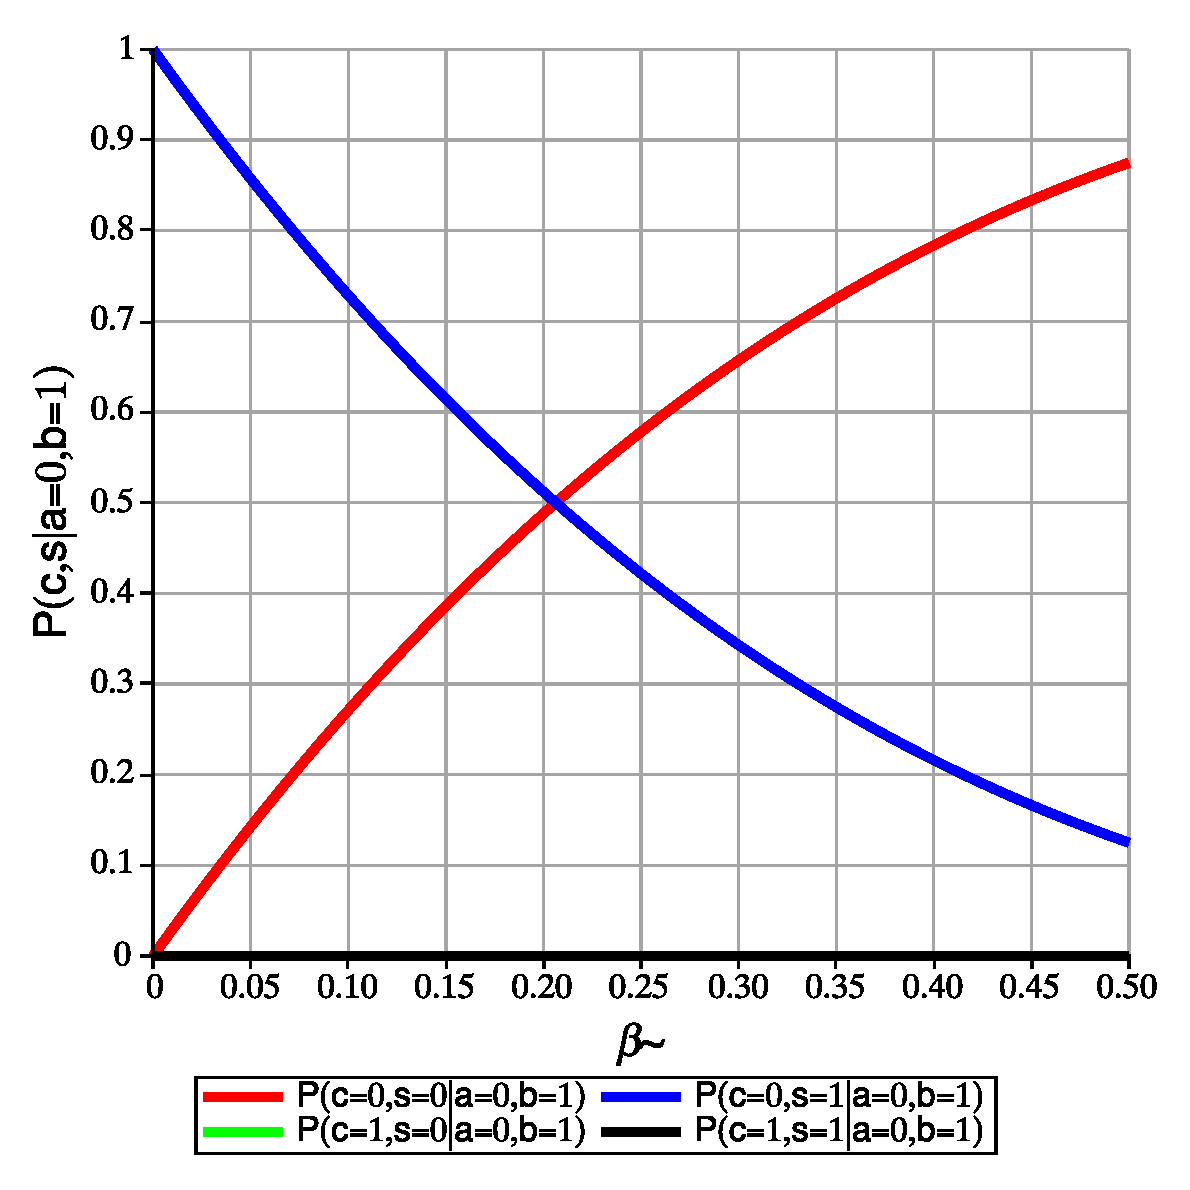
\includegraphics[width=.3\textwidth]{media/noisy_half_adder_value_dist_01.eps}  &
        \includegraphics[width=.3\textwidth]{media/noisy_half_adder_value_dist_11.eps}    \\
        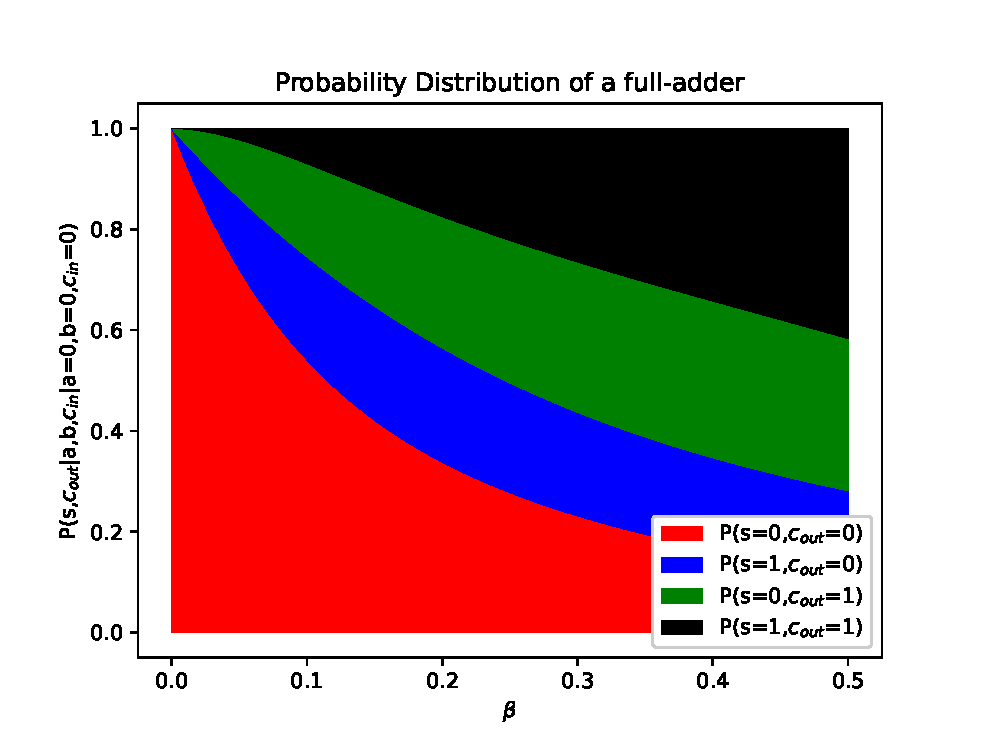
\includegraphics[width=.3\textwidth]{media/noisy_full_adder_value_dist_000.eps} &
        \includegraphics[width=.3\textwidth]{media/noisy_full_adder_value_dist_010.eps} &
        \includegraphics[width=.3\textwidth]{media/noisy_full_adder_value_dist_110.eps}   \\
        \includegraphics[width=.3\textwidth]{media/noisy_full_adder_value_dist_001.eps} &
        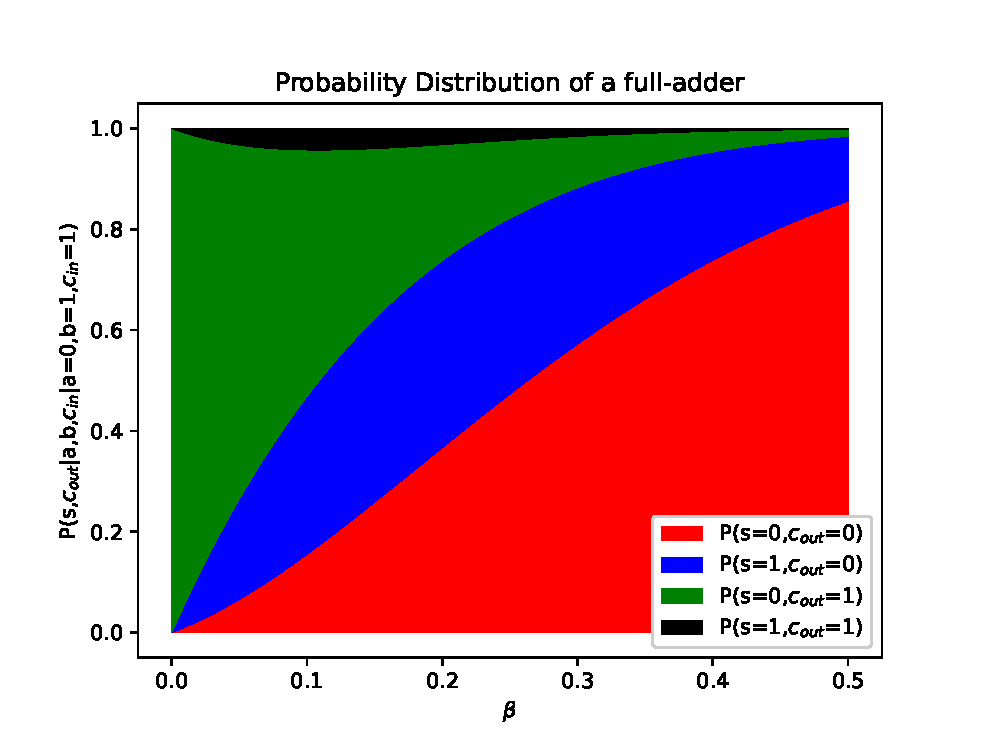
\includegraphics[width=.3\textwidth]{media/noisy_full_adder_value_dist_011.eps} &
        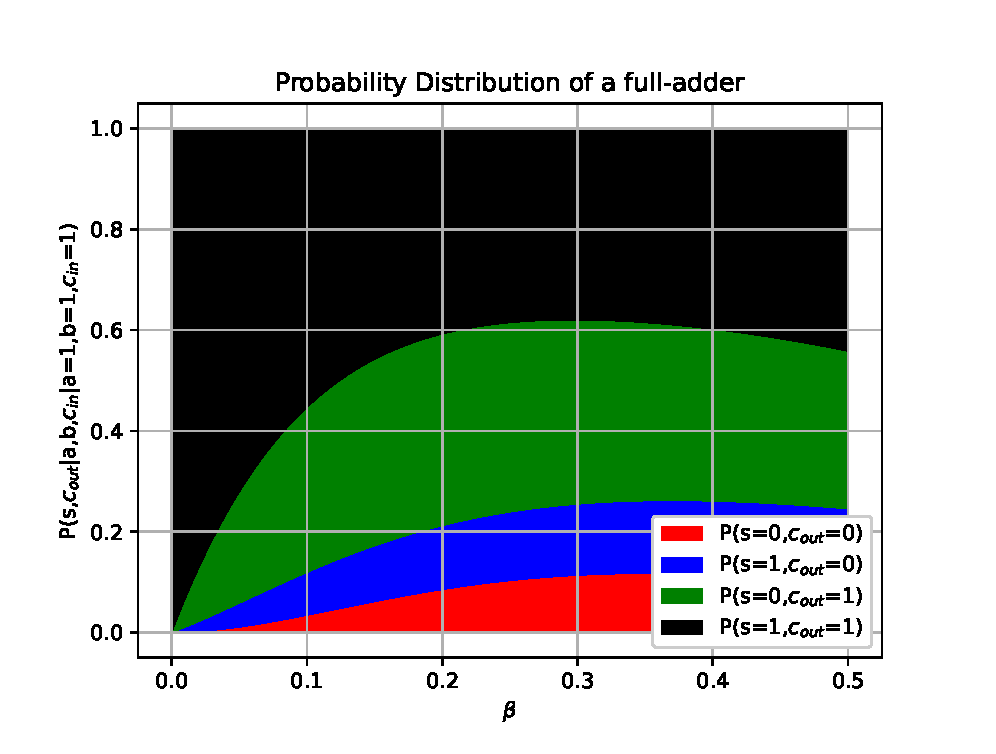
\includegraphics[width=.3\textwidth]{media/noisy_full_adder_value_dist_111.eps}   \\
    \end{tabular}
    \caption{Probability distribution for $P(s,\cout)$ for all distinct inputs for the noisy half-adder (top row) and the full-adder (middle \& bottom row). The graphs show the change of the probability distributions over the four possible outcomes as stack-plots as $\beta$ in (\ref{eq:bit_flip_to_0}) varies from $0$ to $\frac{1}{2}$ and $\alpha = 0$; this case is equivalent to assuming there is only leakage of information due to low-voltage. In all graphs, red denotes $P(s=0,\cout=0)$, blue denotes $P(s=1,\cout=1)$, green denote $P(s=0,\cout=1)$ and black denotes $P(s=1,\cout=1)$. Note that longer computation paths bias towards more errors, for example the plots in the top and middle row should be identical because they have the same truth table. \label{fig:noise_prob_dist}}
\end{figure}

In Figure \ref{fig:noise_prob_dist} we have shown how the distributions of the half-adder and full-adder vary as functions of $\beta$ when $\alpha=0$ (i.e., it is not possible that any of the input bits ever flip erroneously from $0$ to $1$). Similarly, in Figure \ref{fig:noise_prob_dist_4bit_adder} we have shown the distribution of the sum for the 4-bit adder for different values of $\beta$. One thing to note about this induced probability distribution is that, the longer the computation path, the more errors get introduced: for example, the top and middle row of Figure \ref{fig:noise_prob_dist} should have identical distributions as their truth tables are identical but the middle row uses more logic gates as an additional half-adder is used. Also, while the variance of the noisy 4-bit adder is somewhat symmetric, but for more than 10\% of bit-flip noise the right output is not always the most likely anymore.

\begin{figure}
    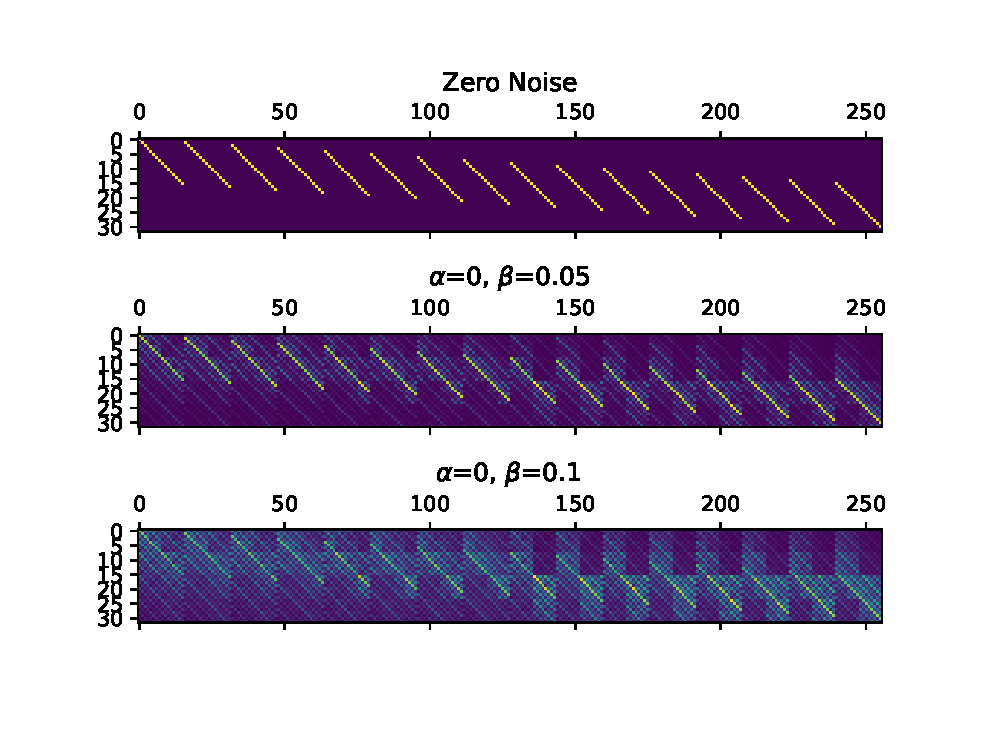
\includegraphics[width=.95\textwidth]{media/noisy_4bit_adder_value_dist_full.eps}
    \caption{Probability distribution for $P(S|A,B)$ for all distinct 256 inputs for the noisy 4-bit adder for increasing values of the noise $\beta$ in (\ref{eq:bit_flip_to_0}). In each of the 3 plots, $S$ takes up to 31 values indexing the $y$-axis and $(A,B)$ take up to 256 values (i.e., the bit-string $a_0a_1a_2a_3b_0b_1b_2b_3$ interpreted as an 8-byte number). \label{fig:noise_prob_dist_4bit_adder}}
\end{figure}

